%!TEX root=../main.tex
\section{Experiments}
\label{sec:experiments}

\begin{figure}[t!]
  \centering
  \begin{subfigure}[b]{0.46\textwidth}
    \caption{Income Prediction.}
    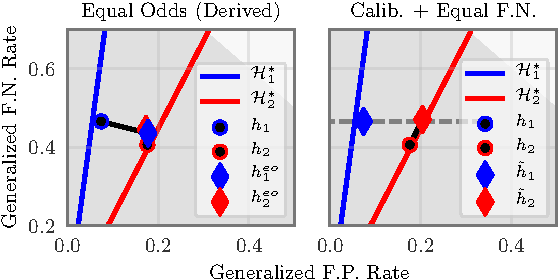
\includegraphics[width=\columnwidth]{figures/adult-fps.pdf}
    \label{fig:adult-res}
  \end{subfigure}
  \quad
  \begin{subfigure}[b]{0.46\textwidth}
    \caption{Health Prediction.}
    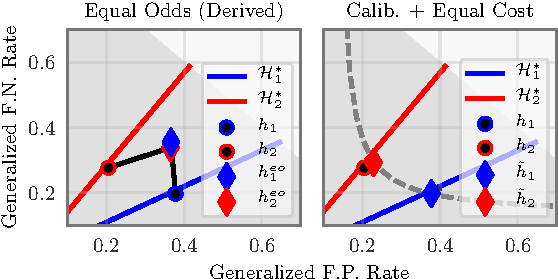
\includegraphics[width=\columnwidth]{figures/health-fps.pdf}
    \label{fig:health-res}
  \end{subfigure}
  \begin{subfigure}[b]{0.67\textwidth}
    \caption{Recidivism Prediction.}
    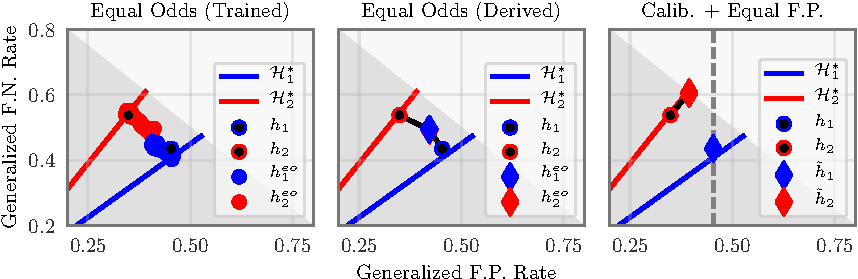
\includegraphics[width=\columnwidth]{figures/compas-fps.pdf}
    \label{fig:compas-res}
  \end{subfigure}
  \vspace{-1.3em}
  \caption{Generalized F.P. and F.N. rates for two groups under
  Equalized Odds and the calibrated relaxation. Diamonds represent post-processed classifiers.
  Points on the Equalized Odds (trained) graph represent classifiers achieved by modifying constraint hyperparameters.}
  \label{fig:res}
\end{figure}

%\gp{New motivation: given that we have a method that produces
  %an optimal CPP classifier, we want to see the minimal trade-off
  %between FP/FN rates that is necessary in order to achieve CPP.}

In light of these findings, our goal is to understand the impact
of imposing calibration and an equal-cost constraint on
real-world datasets. We will empirically show that, in many cases, this will
result in performance degradation, while simultaneously increasing other
notions of disparity.
%
We perform experiments on three datasets: an
income-prediction, a health-prediction, and a criminal
recidivism dataset.  For each task, we
choose a cost function within our framework
that is appropriate for the given scenario.
We begin with two calibrated classifiers $h_1$ and $h_2$
for groups $G_1$ and $G_2$.
We assume that these classifiers cannot be significantly
improved without more training data or features.
We then derive $\fair h_2$ to equalize the costs while maintaining calibration.
The original classifiers are trained on a portion of the data, and then the new classifiers are
derived using a separate holdout set.
To compare against the (uncalibrated) Equalized Odds framework, we derive
F.P./F.N. matching classifiers using the post-processing
method of \cite{hardt2016equality} ({\bf \hardtetal{}}).
On the criminal recidivism dataset, we additionally learn classifiers that directly
encode the Equalized Odds constraints, using the methods of
\cite{zafar2017fairness} ({\bf \zafaretal{}}).
(See \autoref{app:experiments} for detailed training and post-processing procedures.)
%
We visualize model error rates on the
generalized F.P. and F.N. plane.
Additionally, we plot the calibrated
classifier lines for $G_1$ and $G_2$ to visualize model calibration.

\paragraph{Income Prediction.}
  The Adult Dataset from UCI Machine Learning Repository \citep{Lichman:2013}
  contains 14 demographic and occupational features for various people, with the
  goal of predicting whether a person's income is above $\$50,000$.
  In this scenario, we seek to achieve predictions with equalized cost
  across genders ($G_1$ represents women and $G_2$ represents men).
  We model a scenario where the primary concern is ensuring
  equal generalized F.N. rates across genders,
  which would, for example, help job recruiters  prevent gender discrimination
  in the form of
  underestimated salaries.
  Thus, we choose our cost constraint to require equal generalized
  F.N. rates across groups.
  %
  In \autoref{fig:adult-res}, we see that the original classifiers $h_1$ and
  $h_2$ approximately
  lie on the line of calibrated classifiers.
  In the left plot (\hardtetal{}), we see that it is possible to
  (approximately) match both error rates of the classifiers at the cost of $\eo
  h_1$ deviating from the set of calibrated classifiers.
  In the right plot,
  we see that it is feasible to
  equalize the generalized F.N. rates while maintaining calibration.
  $h_1$ and $\fair h_2$ lie on the same
  level-order curve of $\fairconstname$ (represented by the dashed-gray line),
  and simultaneously remain on the ``line'' of calibrated classifiers.
  %In this case, achieving non-disparity requires a slight increase in the F.N.
  %and F.P. rates of $\fair h_2$.
  It is worth noting that achieving either notion of non-discrimination requires
  some cost to at least one of the groups.
  However, maintaining calibration further increases the difference
  in F.P. rates between groups. In some sense, the calibrated framework
  trades off one notion of disparity for another while simultaneously increasing the overall error rates.
  %Equalized Odds in some senses accomplishes a stronger notion of parity, since the
  %classifiers $\eo h_1$ and $\eo h_2$ have approximately the same generalized F.P. and F.N.
  %rates. Note that these rates are not exactly equal because, unlike
  %\methodnameshort{},
  %\hardtetal{} does not weight error rates by the classifier probability.
  %We can also visualize the tradeoffs that must be made to satisfy the
  %constraints of both frameworks.
  %In order to achieve \hardtetal{}, the classifiers deviate substantially from the
  %set of calibrated classifiers. Conversely, in order to match generalized
  %F.N. rates, \methodnameshort{}
  %must increase the generalized F.P. rate of $G_2$.
  %In fact, the generalized F.P. rates of the two groups become more disparate.
  %\gp{is this too negative?}


\paragraph{Health Prediction.}
  The Heart Dataset from the UCI Machine Learning Repository contains 14 processed features
  from 906 adults in 4 geographical locations. The goal of this dataset is to
  accurately predict whether or not an
  individual has a heart condition. In this scenario, we would like to reduce
  disparity between
  middle-aged adults ($G_1$) and seniors ($G_2$).
  In this scenario, we consider F.P. and F.N. to both be undesirable.
  A false prediction of a heart condition could result in unnecessary medical attention, while
  false negatives incur cost from delayed treatment. We therefore utilize the following cost function
  %
  $
    \fairconst{h_t}{t} = r_{fp} h_t(\x) \left(1 - y\right) + r_{fn} \left( 1 - h_t(\x) \right) y,
  $
  %
  which essentially assigns a weight to both F.N. and F.P. predictions.
  In our experiments, we set $r_{fp}=1$ and $r_{fn}=3$.
  %
  In the right plot of \autoref{fig:health-res}, we can see that
  the level-order curves of the cost function form a curved
  line in the generalized F.P./F.N. plane.
  Because our
  original classifiers lie approximately
  on the same level-order curve, little change is required to equalize the costs of
  $h_1$ and $\fair h_2$ while maintaining calibration.
  This is the only experiment in which the calibrated framework
  incurs little additional cost, and therefore could be considered a viable option.
  However, it is worth noting that, in this example, the equal-cost constraint
  does not explicitly match either of the error types, and therefore the two
  groups will in expectation experience different types of errors.
  In the left plot of \autoref{fig:health-res} (\hardtetal{}), we see that it is
  alternatively feasible to explicitly match both the F.P. and F.N. rates while sacrificing
  calibration.

\paragraph{Criminal Recidivism Prediction.}
  Finally, we examine the frameworks in the context of our motivating example: criminal recidivism.
  As mentioned in the introduction, African Americans ($G_1$) receive a disproportionate
  number of F.P. predictions as compared with Caucasians ($G_2$) when automated risk
  tools are used in practice.
  Therefore, we aim to equalize the generalized F.P. rate.
  In this experiment, we modify the predictions made by the COMPAS
  tool \cite{dieterich-northpointe-fairness}, a risk-assessment tool used in practice by the
  American legal system.
  %
  Additionally, we also see if it is possible to improve the classifiers with training-time
  Equalized Odds constraints using the methods of \citet{zafar2017fairness} (\zafaretal{}).
  %
  In \autoref{fig:compas-res}, we first observe that the original classifiers $h_1$ and $h_2$
  have large generalized F.P. and F.N. rates. Both methods of achieving
  Equalized Odds --- training constraints (left plot) and post-processing (middle plot)
  match the error rates while sacrificing calibration.
  However, we observe that, assuming $h_1$ and $h_2$ cannot be improved, it is
  infeasible to achieve the calibrated relaxation (\autoref{fig:compas-res} right).
  This is an example where matching the F.P. rate of $h_1$ would require
  a classifier worse than the trivial classifier $h^{\br_2}$.
  This example therefore represents an instance in which calibration is completely
  incompatible with any error-rate constraints.
  If the primary concern of criminal justice practitioners is calibration
  \cite{dieterich-northpointe-fairness,flores-re-propublica-fair}, then there
  will inherently be discrimination in the form of F.P. and F.N. rates.
  However, if the Equalized Odds framework is adopted, the miscalibrated risk
  scores inherently cause discrimination to one group, as argued in the introduction.
  Therefore, the most meaningful change in such a setting
  would be an improvement to $h_2$ (the classifier for African Americans)
  either through the collection of more data or the use of more salient features.
  A reduction in overall error to the
  group with higher cost will naturally lead to less error-rate disparity.

%\paragraph{Discussion}


